\subsection*{Komplekse tal}
%%
%%
\begin{opgave}[1]{Den komplekse plan}
Tallene er indtegnet på følgende billede.
\begin{figure}[h!]
	\centering
	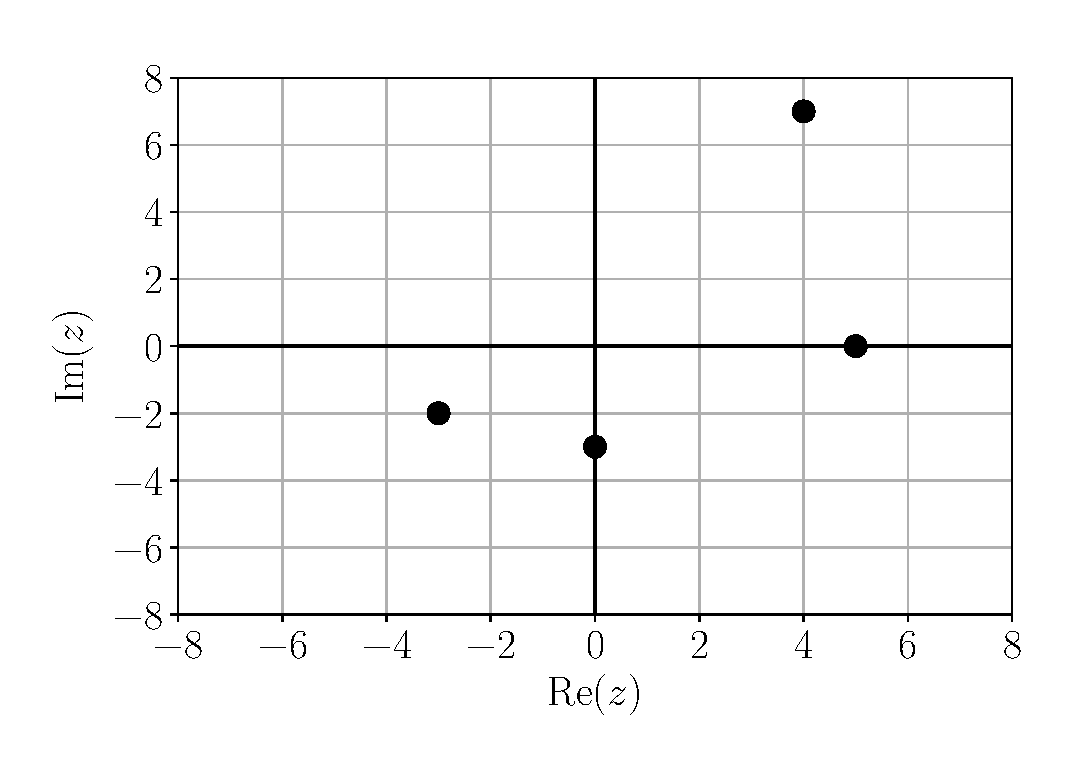
\includegraphics[width=0.6\textwidth]{Matematik/matfig/kompleks_plan.eps}
\end{figure}
\end{opgave}
%%
%%
\begin{opgave}[1]{Regning med komplekse tal}
Her bruges $z_1 = 3+2i, \, \, z_2 = -6+i, \, \, z_3 = 1-5i, \, \, z_4 = -4+3i$.\\
\opg Man får $z_1+z_2 = -3+3i$ og $z_3+z_4 = -3-2i$.
\opg Man får $z_1-z_2 = 9+i$ og  $z_3-z_4 = 5-8i$.
\opg Man får $z_1z_2 = -20-9i$ og $z_3z_4 = 11+23i$.
\opg Man får $z_1/z_2 = -(16/37) - (15/37)i$ og $z_3/z_4 = -(19/25)+(17/25)i$.
\opg Man får $\abs{z_1} = \sqrt{13}$ og $\abs{z_2} = \sqrt{37}$. Endeligt får man, at $\abs{z_3z_4} = \abs{z_3} \abs{z_4} = 5 \cdot \sqrt{26}$.
\end{opgave}
%%
%%
\begin{opgave}[2]{Regneregler for modulus og normkvadratet}
\opg Regnereglerne tages en af gangen. Lad $z_1 = a+bi$ og $z_2 = c+di$.\\ \\
Først \eqref{k-modulus_regneregler1}:
\begin{align*}
\abs{z_1} = \abs{a+bi} = \sqrt{a^2+b^2} = \sqrt{a^2+\left(-b\right)^2} = \abs{a-bi} = \abs{z_1^*} \, .
\end{align*}
Så \eqref{k-modulus_regneregler2}:
\begin{align*}
\abs{z_1z_2} &= \abs{\left(ac-bd\right) + \left(ad+bc\right)i} = \sqrt{\left(ac-bd\right)^2 + \left(ad+bc\right)^2} = \sqrt{\left(ac\right)^2 + \left(bc\right)^2 + \left(ad\right)^2 + \left(bc\right)^2} \\
&= \sqrt{\left(a^2+b^2\right) \cdot \left(c^2+d^2\right)} = \sqrt{a^2+b^2} \cdot\sqrt{c^2+d^2} = \abs{z_1}\abs{z_2} \, .  
\end{align*}
Endeligt \eqref{k-modulus_regneregler3}. Her bemærker man først at
\begin{align*}
\abs{z_1^n} = \abs{\left(z_1^{n-1}\right)z_1} = \abs{z_1^{n-1}}\abs{z_1} \, , 
\end{align*}
hvor \eqref{k-modulus_regneregler2} er brugt i  den anden lighed. Man kan da lave samme trick for $z_1^{n-1}$
\begin{align*}
\abs{z_1^{n-1}} = \abs{\left(z_1^{n-2}\right)z_1} = \abs{z_1^{n-2}}\abs{z_1} \, ,
\end{align*}  
hvilket viser at
\begin{align*}
\abs{z_1^n} = \abs{z_1^{n-1}}\abs{z_1} = \abs{z_1^{n-2}}\abs{z_1}\abs{z_1} \, .
\end{align*}
Ideen er da blot at fortsætte på samme vis, hvilket giver det ønskede resultat. Streng taget burde dette laves som et \emph{induktionsbevis}, hvis det skulle være helt matematisk korrekt, men metoden her er mere intuitiv og illustrerer ideen i beviset.
\opg Her vises formel \eqref{k-normkvadrat2}. Lad $z=a+bi$.
\begin{align*}
\abs{z}^2 = \left(\sqrt{a^2+b^2}\right)^2 = a^2+b^2 = \left(a+bi\right)\left(a-bi\right) = zz^* \, .
\end{align*}
\end{opgave}
%%
%%
\begin{opgave}[2]{Komplekse ligninger}
\opg Der løses for $z$ som i en normal ligning.
\begin{align*}
\frac{z-2}{z+1} = 3i \quad &\implies \quad z-2 = 3i\left(z+1\right) = 3i \cdot z + 3i \quad \implies \quad z - 3i \cdot z = 2 + 3i \\
&\implies z  \left(1-3i\right) = 2+3i \quad \implies \quad z = \frac{2+3i}{1-3i} = -\frac{7}{10} +  \frac{9}{10}i \, .
\end{align*}
\opg Her bruges en anden metode end i 1), for at vise at komplekse ligninger kan løses på forskellige måder. Ideen er at skrive $z=a+bi$, hvor man ikke kender $a$ og $b$ endnu. Dette indsættes i venstresiden af ligningen, og der reduceres
\begin{align*}
z + 3z^* = a+bi + 3(a-bi) = 4a -2bi \, .
\end{align*}
Sammenligner man da med højresiden af ligningen, $5-6i$, giver dette to normale ligninger, da realdelen af venstresiden må være lig med realdelen af højresiden og ligeledes for imaginærdelene. Altså får man ligningerne:
\begin{align*}
4a = 5 \qquad \text{og} \qquad -2b = -6 \, .
\end{align*}
Disse ligninger har løsningerne $a=5/4$ og $b=3$, og løsningen af den komplekse ligning er da
\begin{align*}
z = \frac{5}{4} + 3i \, .
\end{align*}
\end{opgave}
%%
%%
\begin{opgave}[3]{Eulers formel og komplekse tal på polær form}
\opg De komplekse tal for de forskellige værdier af $x$ bliver:
\begin{align*}
e^{i \cdot 0} = 1 \, , \qquad e^{i \cdot \frac{\pi}{2}} = i \, , \qquad e^{i \cdot \pi} = -1 \, , \qquad e^{i \cdot \frac{3\pi}{2}} = -i \, .
\end{align*}
Altså bevæger $e^{ix}$ sig rundt mod uret i den komplekse plan, når $x$ vokser.
\opg Fra Eulers formel har man at
\begin{align*}
\abs{e^{ix}} = \abs{\cos(x) + i \sin(x)} = \sqrt{\cos^2(x) + \sin^2(x)} = \sqrt{1} = 1 \, .
\end{align*}
Altså  er modulus af $e^{ix}$ konstant og ændres derfor ikke, når man ændrer $x$.
\opg Her kan man bruge de samme $x$ som fra 1). Det giver
\begin{align*}
e^{-i \cdot 0} = 1 \, , \qquad e^{-i \cdot \frac{\pi}{2}} = -i \, , \qquad e^{-i \cdot \pi} = -1 \, , \qquad e^{-i \cdot \frac{3\pi}{2}} = i \, .
\end{align*}
Altså bevæger $e^{-ix}$ sig rundt med uret i den komplekse plan, når $x$ vokser.
\opg Fra Eulers formel har man at
\begin{align*}
\abs{e^{-ix}} = \abs{\cos(-x) + i \sin(-x)} = \abs{\cos(x) - i \sin(x)} = \sqrt{\cos^2(x) + \left(-\sin(x)\right)^2} = \sqrt{1} = 1 \, ,
\end{align*}
hvor det er benyttet at $\cos(-x) = \cos(x)$ og at $\sin(-x) = -\sin(x)$. Dette skyldes at cosinus er en lige funktion, mens sinus er en ulige funktion. Altså  er modulus af $e^{-ix}$ konstant og ændres derfor ikke, når man ændrer $x$.
\opg Først bemærkes det, hvis man tegner $z=a+bi$ i den komplekse plan, at man vha. $z$'s modulus, $\abs{z}$, og argument, $\theta$, kan skrive $a$ og $b$ som følger
\begin{align*}
a = \abs{z} \cos(\theta)  \qquad \text{og} \qquad b = \abs{z}\sin(\theta) \, .
\end{align*}
Bruger man da Eulers formel, får man at
\begin{align*}
z = a+bi = \abs{z}\cos(\theta)+i\abs{z}\sin(\theta) = \abs{z}\left(\cos(\theta)+i\sin(\theta)\right) = \abs{z}e^{i\theta} \, .
\end{align*}
\end{opgave}
%%
%%
\begin{opgave}[3]{Komplekse tal og lys i materialer}
k
\end{opgave}